% %
% LAYOUT_E.TEX - Short description of REFMAN.CLS
%                                       99-03-20
%
%  Updated for REFMAN.CLS (LaTeX2e)
%
\documentclass[twoside,a4paper]{refart}
\usepackage{makeidx}
\usepackage{ifthen}
\usepackage{graphicx}
\usepackage{listings}
\usepackage{color}
\lstset{
	basicstyle=\footnotesize,
	stringstyle=\color{red},
	keywordstyle=\color{blue},
	rulecolor=\color{black}
} 
% ifthen wird vom Bild von N.Beebe gebraucht!

\def\bs{\char'134 } % backslash in \tt font.
\newcommand{\ie}{i.\,e.,}
\newcommand{\eg}{e.\,g..}
\DeclareRobustCommand\cs[1]{\texttt{\char`\\#1}}

\title{A User Manual for Simulate, Aggregate, and Validate Components of the GWAS/QTL Tool Validation Workflow}
\author{Ann Stapleton and Dustin Landers \\
University of North Carolina Wilmington \\
}

\date{}
\emergencystretch1em  %

\pagestyle{myfootings}
\markboth{Validate: A Workflow for Evaluating GWAS/QTL Tools}%
         {Validate: A Workflow for Evaluating GWAS/QTL Tools}

\makeindex 

\setcounter{tocdepth}{2}

\begin{document}

\maketitle

\tableofcontents

\newpage

%%%%%%%%%%%%%%%%%%%%%%%%%%%%%%%%%%%%%%%%%%%%%%%%%%%%%%%%%%%%%%%%%%%%

%\begin{center}
%	\makebox[12cm][r]{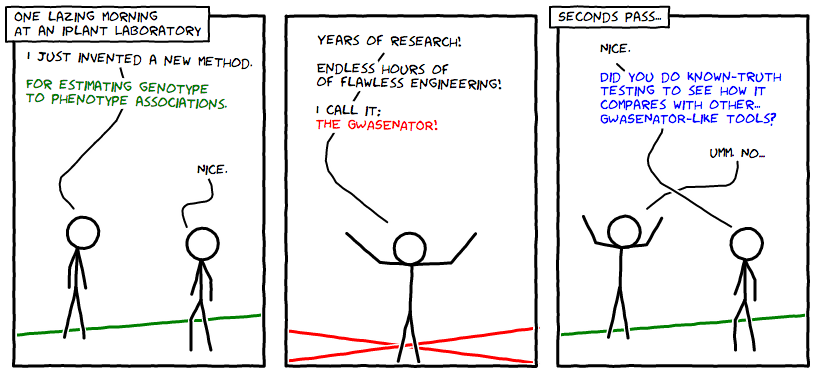
\includegraphics[width=17cm]{doc_comic1}}
%\end{center}

\section{Introduction}

\subsection{About the Developers}

\marginlabel{Project Lead and Principal Investigator}Dr. Ann Stapleton works at the interfaces, such as the junctions between research and teaching, individual research projects and large collaborative projects, the organization of international meetings and high-school teacher inquiry labs. Most recently, she has worked at the interface between plant biology and software engineering, leading the way to broad methods applicable to evaluating genotype-to-phenotype analytical methods.

\marginlabel{Statistical Analyst and Developer}Dustin Landers received a BS from Appalachian State where he learned a lot about survey research and using statistics to solve problems and answer questions. He continued his education at UNCW by studying Applied Statistics. Moving from world of polling and survey statistics to the that of Big Data, he has an interest in bridging the gap between statistics and software engineering and seeing the combined discipline brought to bear on problems once considered impossible.

\index{author}

\subsection{Why Validate?}

To test known-truth data sets, we originally weren't sure of the best way to approach the problem. We had the idea of using ROC plots. We wanted to look at true positive rates, false positive rates and accuracy. Of course, this was never really feasible because any one simulation run could be atypical, and all of these methods could only analyze a single simulation run. We asked ourselves how could we run lots of simulations through a tool, and test the outputs in a way that gave us insight in to the performance of these GWAS and QTL tools?

We decided that in order to allow lots of simulations to be tested, we needed a method that that allowed iterations over hundreds or even thousands of simulation-runs. This birthed the idea of Validate, which is a tool that returns these sorts of measures of tool success for massive amounts of outputs.

But how do we run all these simulations? How do we store them all in a single location so we can calculate these measures? How do we visualize them?

These are the problems we sought to solve. For each problem, we have our own solution. We also left them divided. This way you can decide whether to use our solution or to use your own if you have a unique scenario.

\subsection{Getting iPlant Credentials}

\subsection{Getting Your Application on an API or on an Atmosphere Image}

\subsection{Where Can I Get These Softwares?}

\subsection{How to Use This Manual}
We assume that you have a statistical GWAS/QTL tool of some kind. We will refer to this as your "box". This is to make the language easier to understand as you progress through this manual.

We also assume that you are at least a little bit comfortable with using the command-line, as both using an Atmosphere image or an API will involve a decent amount of this. However, we will try our best in this manual to be simple and straight-forward so that you don't have to be a command-line veteran to use this workflow.

\begin{enumerate}
\item \textbf{Install your box on one of iPlant's API's or on an Atmosphere image.}
\seealso{Section 1.4}
\item \textbf{Develop simulations or use existing simulations.}
\seealso{Section 2}
\item \textbf{Run simulations through your box.}
%\seealso{Section 4}
%\vspace{-1.3mm}
\item \textbf{Aggregate your box's results files to a folder or series of folders.}
%\seealso{Section 5}
\item \textbf{Run Validate on your aggregated folder.}
\item \textbf{Download your data, merge, and visualize.}
\end{enumerate}

%\newpage
\section{Develop simulations}

%\index{layout design}

\subsection{Building simulations with Simulate in Atmosphere}

Using Simulate is pretty straightforward. If you are using an Atmosphere image, you should have begun the testing process by launching the Validate Atmosphere image so that you have Simulate, Aggregate, and Validate already in your image for testing.

Simulate uses the powerful python package called simuPOP-- which is a coalescent forward-in-time simulation process that essentially uses defined initial settings and evolves the population over a series of generations. The resulting genotypes are generally realistic in their distributions. Simulate goes a step past this and provides models for quantitative trait generation based on several factors that you can provide. 

With Simulate, you specify:
\begin{itemize}
\item Verbose mode [-v or --verbose]
\item Population size/s [-s or --size]
\item Genome size/s [-n or --number]
\item The loci with effects [-l or --loci]
\item The size of these effects [-e or --effect]
\item A heritability variable between 0 and 1 [-i or --heritability]
\item Population mean/s [-m or --mean]
\item The number of generations to evolve [-g or --gen]
\item The recombination rate [-r or --rrate]
\item The filename you want files to be saved as [-f or --filename]
\end{itemize}

You access the Simulate tool from the command-line in the Atmosphere terminal emulator. Use (python Simulate.py --help) to see all the usages above. Heritability is defined as the amount of phenotypic variance explainable by a purely genetic model. It is only approximated in Simulate by tuning the phenotype variance until a polynomial model predicts a relatively close $R^2$ value for a linear model with only genetic variables.

For example, suppose you wanted to have two sub-populations, with 1000 individuals each, 3000 markers per individual and only the first three loci have effects of 0.2 each. The population mean is 2.7 for both populations and you want to evolve the populations for 100 generations. Also, suppose you wanted to have a heritability of about 0.25. The following code would generate a single simulation.

%\begin{center}
\begin{lstlisting}[frame=single]
$ python Simulate.py --verbose -s 1000,1000 -n 3000 -l 0,1,2 
+	-e 0.2,0.2,0.2 -i 0.25 -m 2.7 -g 100 
+	--filename test_dataset
\end{lstlisting} 
%\end{center}

As you can see, either long-flags such as those beginning with -- or short-flags (those beginning with -) can be used and in any order. We recommend the option -v or --verbose at some point so you can see Simulate progress as it generates the simulation.

One other thing to note is that anytime multiple arguments are allowed for a flag (such as the population sizes), a single comma is used to separate them. It is also important that this comma separator does not include spaces.

Also, we will show an example of using Simulate to generate multiple simulations from a single command. This would be because the phenotypes are inherently generated from a probability distribution, so multiple simulations may be needed to get accurate validations of statistical tools.

To generate 10 different simulations from the command-line:

\begin{lstlisting}[frame=single]
$ for i in {1..10};
$ do echo "Generating simulation $i";
$ python Simulate.py --verbose -s 1000,1000 -n 3000 -l 0,1,2 
+	-e 0.2,0.2,0.2 -i 0.25 -m 2.7 -g 100 
+	--filename test_dataset$i;
$ done;
\end{lstlisting} 

It may also be worth mentioning that a single population could be written as just (-s 1000). And (-m) can be used either as one argument or the length of arguments given for (-s). For example, if you have three sub-populations like so (-s 1000,1000,1000) then -m can be written as (-m 1.3) for a single mean or as (-m 1.2,1.3,2.7) as three different sub-population means. 

\section{Run Simulations}
\subsection{Running simulations through your box on Atmosphere}
After you have installed your box on a Validate Atmosphere image, you need to get the simulations in the appropriate format and then simply execute them from the command-line. A tool provided on the iPlant Discovery Environment as well as the iPlant Foundation API system called PLINK-Conversion allows the quick conversion in to other popular formats. However, the use of PLINK-Conversion and its full documentation is outside of the scope of this manual.

In order to execute the simulations through your box in Atmosphere, you must first install your box locally and then simply execute from the command-line. This can be done using a similar for-loop process. An example of this may be:

\begin{lstlisting}[frame=single]
$ for i in {1..5};
$ do echo "Testing BOX with simulation $i";
$ mybox --ped test$.ped --map test$i.MAP
$ done;
\end{lstlisting} 

\section{Aggregate Results}
\subsection{Aggregate results using the Aggregate software on the Validate Atmosphere image}

The Aggregate software is the one GUI tool available in the Validate workflow. This may be an unnecessary step if you have been testing your box completely from an Atmosphere image. Other users who have been testing from the API system, may find that individual analyses are now grouped in folders in a common folder (most likely your username/analyses folder). In this case, a good option at this point is to make sure that your actual results files (for which you will run Validate on) are located somewhere in a common folder. Each folder will provide a separate analyses folder. 

In other words, if all your results files are already located in a single location, then you can skip this step and move on to the heading "Run Validate."

To run Aggregate, simply type from the command-line:

\begin{lstlisting}[frame=single]
$ python Aggregate.py
\end{lstlisting} 

\textbf{Step 1) Enter username and password.}

First, you need to enter your iPlant credentials in the indicated lines.

\textbf{Step 2) Enter the folder location where all your tool analyses are located and click \textit{View Folders in Directory}.}

Now, you need to type the out the full location of the folder starting with username where your analyses are located. For example, if you ran all your simulations through your box using either the Discovery Environment or an API system, then it is most likely that your results are all stored in individual folders in \textit{your-username/analyses}.

\textbf{Step 3) Select only folders from the known-truth data sets runs.}

By clicking this button, you should now see a list of all folders and files in that directory. You now need to select the folders that you want to further view in order to obtain the results files needed. You can use Control + Click to select individual folders or Shift + Click in order to select longer lists of folders. Once they are highlighted, you need to click the select button to reduce the list to just those you want to look further in to.

There is also a "Select All Containing:" button at the bottom of the list. So if all of your analyses contain the word "MyBox" then you can easily select just those results directories by using this option.

\textbf{Step 4) Click \textit{View Contents of Selected Folders}}

Once you've got all your folders in the first listbox, click the button on the right call \textit{View Contents of Selected Folders} and this will iterate over the folders in the left-most listbox and add the contents of all those folders to the right-most listbox. It should take a few minutes, so give it some time. Once its done, see if you can spot the files that you were interested in moving.

As you can see, every single item in the right-most listbox is a file or folder contained with \textit{one} of the folders in the left-most listbox. Now, we need to select all the files from the right-most listbox that we wish to move to the folder we created in order to run \textit{Validate}.

\textbf{Step 5) Select just the tool outputs from the right-most listbox.}

In order to select just the right files that you intend to move, you can use the same \textit{Select All Containing:} logic button we used earlier, or if they all have the same file extension then we can use another option.

Above the right-most listbox is a button labelled \textit{Select File Type}. Next to that, we can type the common extension of our box's results files and use this to select what we want.

\textbf{Step 6) Move the files to your \textit{Validate} analysis folder or some common folder.}

Now, we can move the files. In the text box next to the \textit{Move Files} button enter the full path of the folder we want to move them to. In our case, we named it \textit{my\_Validate\_analysis} so we would enter in to the text box: \textit{dalanders/analyses/my\_Validate\_analysis}. Then click \textit{Move Files} in order to begin iterating over that list and sending the \textit{.qassoc} files to the folder you created. It is not necessary for the folder to already exist, the Aggregate application will create the folder automatically if it does not exist.

This process can take about as long or longer than it did to actually view the files. Keep in mind, that this process uses the iPlant Foundation API system, so for each item in the right-most list, a request is send to the API to move that file to the folder you specified. 

It may also be worth noting that by the time you read this manual, this could be a fully-integrated step in the iPlant Discovery Environment, as there was talk about this functionality being available given more time. However, we found it necessary, even though this part of the problem is almost entirely logistical, to be able to select files from multiple files and move them in to a single aggregate folder.

\section{Running Validate} 

\section{Visualizing the Validation}

\section{Acknowledgements}

\section{How to Interpret Performance Measures}
\subsection{AUC}
\subsection{H}
\subsection{KS}
\subsection{TPR}
\subsection{FPR}
\subsection{Accuracy}
\subsection{MAE}
\subsection{RMSE}
hmeasure.net

\end{document}